\newpage
\begin{center}
  \textbf{\large 1. Аналитический обзор }
\end{center}
\refstepcounter{chapter}
\addcontentsline{toc}{chapter}{1. Аналитический обзор }

\section{Проблема робастности моделей машинного обучения в изменяющихся условиях среды}

       В области методов машинного обучения, применяемых в робототехнике, наибольший интерес представляют подходы, применимые в реальных условиях с высокой эффективностью. Выделяют два основных направления для обучения таких моделей: на реальных данных и на синтетических данных в симуляторе. 
    
    При использовании реальных данных, динамика среды остается неизменной, как на этапе обучения, так и на этапе эксплуатации, поэтому модель может быть успешно обучена, например методами имитационного обучения \cite{jang2017end, levine2018learning}. Однако, данный подход содержит несколько ограничений: во-первых, сбор реальных данных может быть ресурсоёмким и небезопасным; во-вторых, сложно обеспечить достаточное покрытие пространства состояний среды. Поэтому второй подход, основанный на обучении в симуляторе, является более предпочтительным, так как данные в симуляторе дешевые, а взаимодействие агента со средой и сбор данных не угрожает реальному оборудованию. Большинство научных работ применяют этот подход для создания моделей с помощью обучения с подкреплением, имитационного обучения и других методов машинного обучения. Несмотря на преимущества, основной проблемой данного подхода является так называемая проблема sim-to-real gap \cite{he2023bridging}, связанная с тем, что симулятор представляет собой аппроксимацию реального мира, и его динамика отличается от реальной. Это приводит к тому, что модель во время обучения на данных из симулятора, учится оперировать в мире с одной динамикой, а затем запускается в условиях другой. Формально это можно описать как изменение функции перехода состояний \cite{josifovski2024continual}.

    Существует множество решений описанной проблемы такие как: идентификация системы, доменная рандомизация, доменная адаптация и другие. Концептуальные иллюстрации основных подходов представлены на рис.~\ref{sim-to-real-app}. Подход доменной рандомизации обладает большей популярностью ввиду его простоты. Суть подхода подразумевает создание разнообразных сценариев обучения, путём варьирования параметров симуляции, таких как: физические и визуальные характеристики объектов и окружающей среды, освещение, кинематические и динамические параметры робота и другие. В таком случае, предполагается, что среда реального мира -- это лишь одна из вариаций исходной среды симулятора. Если модель будет эффективной на распределении вариаций сцен, генерируемой доменной рандомизацией, то она будет эффективна и в реальных условиях. Таким образом доменная рандомизация решает проблему sim-to-real, делая модель более робастной по отношению к различным сценариям.  


    \begin{figure}[!t]
      \centering
      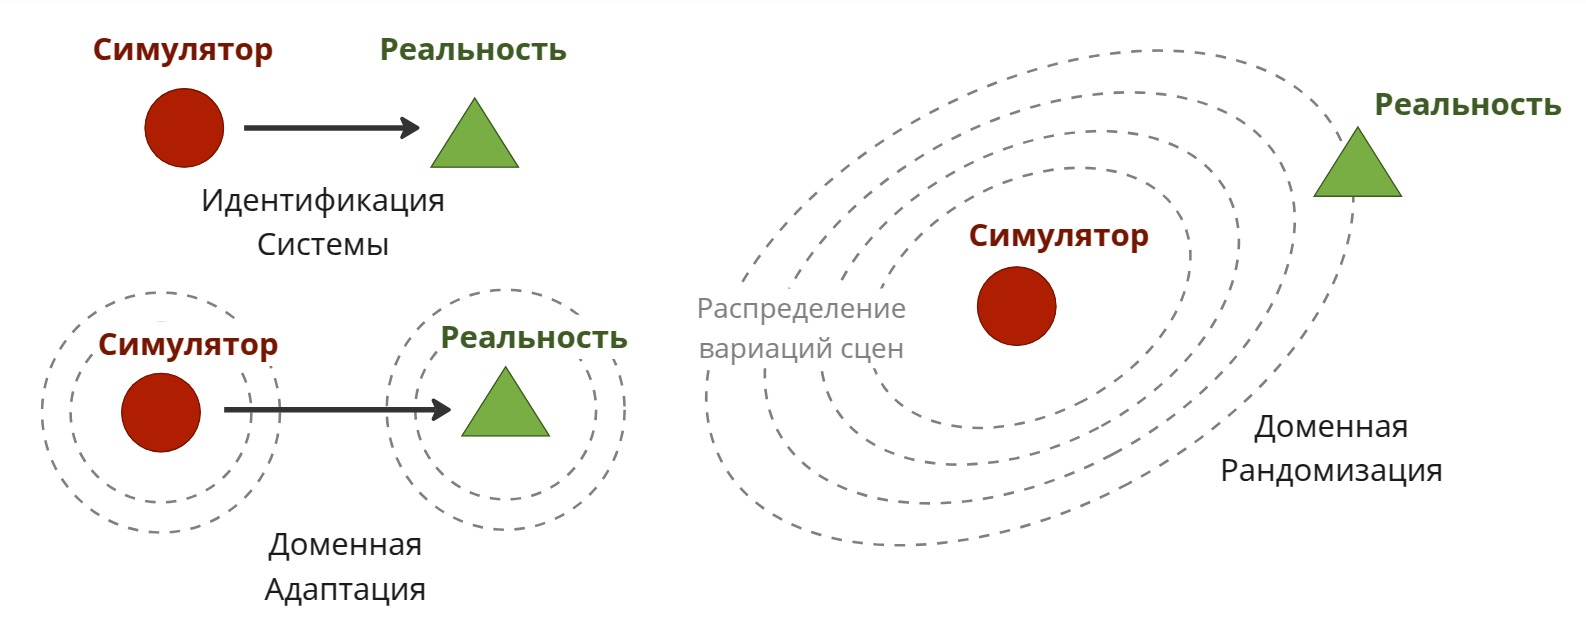
\includegraphics[width=150mm]{images/sim2real.jpg}
      \caption{Концептуальные иллюстрации подходов к решению проблемы sim-to-real
      }
      \label{sim-to-real-app}
    \end{figure}

    На примере доменной рандомизации можно сделать вывод, что свойство модели сохранять эффективность в средах с различными параметрами предсказывает успех решения проблемы sim-to-real. Действительно, в работе SIMPLER \cite{li24simpler} было показано, что эффективность модели в реальном мире коррелирует с усредненной эффективностью модели на различных вариациях симуляционной среды. Таким образом, требование робастности необходимо для запуска модели в реальных условиях. 

    Еще одна причина, по которой робастность является ключевым требованием, обусловлена высокой степенью нестационарности, стохастичности и неопределенности среды реального мира. Это проявляется в изменении входных данных, шумов, распределений, на которых обучалась модель. Такие изменения могут быть вызваны как внешними факторами (например, изменением освещения или вмешательство человека), так и внутренними процессами (изменением конфигурации системы или изнашиванием оборудования). В работах \cite{li24simpler, pumacay2024colosseum} было показно, что эффективность моделей в симуляторе коррелирует с эффективностью в реальных условиях при варьировании одних и тех же параметров. Поэтому важно, чтобы обученная политика была робастной, то есть сохраняла показатели эффективности при изменении параметров среды, адаптировалась к новым условиям и демонстрировала устойчивость к возмущениям, что является критическим аспектом для успешного развертывания моделей машинного обучения в реальных условиях.

    Таким образом можно выделить две основные причины, по которым робастность является решающим требованием к моделям машинного обучения при запуске в условиях реального мира:

    \begin{enumerate}
        \item Большинство моделей обучаются на синтетических данных симулятора, робастность обученных таким образом моделей, имеет сильную корреляцию с эффективностью моделей в реальном мире
        \item Робастность модели позволяет сохранять эффективность при изменяющихся условиях, присущих реальному миру
    \end{enumerate}
    
    Недавние работы описывающие методы с применением машинного обучения показывают впечатляющее результаты в решении манипуляционных задач \cite{shridhar2022peract, goyal2023rvt, goyal2024rvt2, rt12022arxiv, rt22023arxiv}. Однако, большинство работ проводят оценку эффективности моделей на условиях, близких к обучающим, или с минимальным варьированием параметров среды, такими как рандомизация положения объектов манипулирования. Подобный подход оценивания не позволяет сделать вывод об обобщающей способности моделей. Поэтому возникает необходимость в методе, который бы позволял оценивать робастность моделей по отношению к варьированию параметров среды.

\section{Современные методы оценки робастности моделей}

    \subsection{The COLOSSEUM}

    Одним ярким примером такого метода для оценки робастности моделей является работа The COLOSSEUM \cite{pumacay2024colosseum}, целью которого является определение падения эффективности моделей при изменении параметров среды. Метод предоставляет собой программный модуль на базе платформы RLBench \cite{james2020rlbench} позволяющий варьировать 14 параметров среды, среди которых цвета, текстуры объектов, параметры освещения и другие. Изменяя описанные параметры можно изменить распределение выходных данных: $p(x_{test}) \neq p(x_{train})$, но при этом условная вероятность распределения действий остается такой же: $p(y_{test} | x_{test}) = p(y_{train} | x_{train})$. Эффективность моделей оценивается долей успешных эпизодов, где успех эпизода определяется задачей. Алгоритм работы метода можно описать следующим образом:

    \begin{enumerate}
        \item Генерация обучающего набора данных на исходной, не рандомизированной среде
        \item Обучение модели на сгенерированных данных, робастность которой будет оценивается
        \item Тестирование обученной модели в среде, с последовательным варьированием каждого из 14 параметров 
        \item Для каждого параметра производится расчет падения доли успешных эпизодов относительно доли успешных эпизодов на исходной, не рандомизированной среде
        \item Определению ключевых для работы модели параметров, варьирование которых сильнее других влияет на эффективность модели
    \end{enumerate}

    По данному алгоритму авторы работы оценили робастность 5 передовых моделей для манипуляции: R3M \cite{nair2022r3m}, MVP \cite{Radosavovic2022}, PerAct \cite{shridhar2022peract}, RVT \cite{goyal2023rvt}, VoxPoser \cite{huang2023voxposer}. По результатам, доля успешных эпизодов падает на $30-50\%$ при варьировании параметров среды, и на более $75\%$ при применении всех вариаций. Оказалось, что рассматриваемые модели наиболее уязвимы по отношению к параметрам освещенности, цвету объекта манипулирования и количеству отвлекающих объектов. 

    \subsection{KitchenShift}
        Аналогичный метод предоставляют авторы работы KitchenShift \cite{xing2021kitchenshift}. Отличие от работы The COLOSSEUM заключается в количестве параметров доступных для вариации, в данной работе их 7, среди которых: 3D модели и текстуры объектов, положение камеры, освещение, начальное состояние объектов и робота. Алгоритм:

        \begin{enumerate}
            \item Модель обучается задаче $\mathcal{T}_{train}$ в домене $\mathcal{D}_{train}$ с доступом к ограниченному набору демонстраций
            \item Производится тестирование модели на задаче $\mathcal{T}_{train}$ на множестве доменов $\{\mathcal{D}_{shifted}\}$, которые были получены варьированием параметров среды.
        \end{enumerate}

    Согласно этому алгоритму, были оценены методы на основе имитационного обучения, по результатам метрики эффективности моделей значительно снизились под воздействием новых, смещенных параметров среды.

    \subsection{SIMPLER}

        Рассмотренные ранее работы предполагают обучения моделей, за которым следует тестирование. Однако, иногда требуется оценить робастность уже обученных моделей.
        Авторы работы SIMPLER \cite{li24simpler} предлагают решение данной проблемы, в контексте моделей, обученных на реальных данных. В таком случае, не целесообразно проводить тестирование в реальных условиях, так как это небезопасно и ресурсоемко, поэтому необходимо проводить валидацию в симуляторе. Стоит отметить, что в работах The COLOSSEUM и KitchenShift отличие между доменами $\mathcal{D}_{train}$ и $\mathcal{D}_{shifted}$ заключается в изменении одного или нескольких параметров симулятора, поэтому на этапе тестирования изменение эффективности модели по большому счету обусловлено исключительно влиянием варьируемого параметра. В случае с моделью, обученной на реальных данных, нужно обоснование, почему изменение эффективности модели в симуляторе было вызвано изменяемым параметром. Для того чтобы уменьшить рассогласование между сценой симулятора и реальным миром, были применены инструменты real-to-sim для создания реалистичной среды с точки зрения визуальных и физических составляющих. Эмпирическим путем было установлено, что эффективность модели в построенной сцене коррелирует с эффективностью модели в реальном мире при одних и тех же изменениях в параметрах. Таким образом, данная работа показывает, что в симуляторе можно оценивать изменение эффективности при варьировании параметров, даже для моделей обученных на реальных данных. 

    Наиболее перспективной является работа The Colosseum, так как она обладает большой масштабируемостью, а также включает в себя большее количество возможных рандомизаций. Также этим методом были исследованы передовые модели, эффективность которых заметно снизилась в других условиях, что говорит об актуальности данного подхода.
    
\section{Обзор симуляционных платформ для тестирования робастности моделей}

    В данном разделе будут рассмотрены перспективные симуляторы для построения метода оценки робастности.

    \subsection{IsaacSim}
    IsaacSim \cite{nvidia_isaac_sim} -- это высокопроизводительная платформа для симуляции и обучения роботов, разработанная NVIDIA. Она позволяет проводить параллельное обучение агентов в виртуальных средах с использованием графических процессоров (GPU). Основные особенности IsaacGym включают:
    \begin{itemize}
        \item Поддержка физически точных симуляций с использованием движка PhysX.
        \item Возможность одновременного обучения тысяч агентов в одной среде.
        \item Высокая фото-реалистичность.
    \end{itemize}
    
    Инструменты предоставляемые IsaacSim позволяют создавать реалистичные сцены, которые упрощают решение проблемы sim-to-real и позволяют проводить оценку моделей, обученных на реальных данных, по примеру работы SIMPLER.
    
    \subsection{RLBench}
    RLBench \cite{james2020rlbench} -- это платформа для обучения с подкреплением, ориентированная на задачи манипуляции роботами. Она предоставляет набор из более чем 100 задач, таких как открывание дверей, перемещение объектов и сборка конструкций. Особенности RLBench включают:
    \begin{itemize}
        \item Большой набор предопределенных задач, которые можно использовать для тестирования и обучения моделей.
        \item Возможность генерации данных для обучения и тестирования моделей.
    \end{itemize}
    RLBench позволяет оценивать робастность моделей в условиях, близких к реальным, благодаря разнообразию задач и сценариев.
    
    \subsection{MuJoCo}
    MuJoCo \cite{todorov2012mujoco} -- это физический движок, широко используемый для моделирования сложных динамических систем. Основные преимущества MuJoCo:
    \begin{itemize}
        \item Высокая точность моделирования физических взаимодействий, включая контакты, трение и деформации.
        \item Возможность гибкой настройки параметров среды.
    \end{itemize}
    MuJoCo является одной из наиболее популярных платформ благодаря своей гибкости и точности.

    Каждая из рассмотренных платформ имеет свои уникальные особенности, однако, для задачи оценивания робастности наиболее уместным является симулятор IsaacSim, ввиду его повышенной точности и качества графики. 